% Options for packages loaded elsewhere
\PassOptionsToPackage{unicode}{hyperref}
\PassOptionsToPackage{hyphens}{url}
%
\documentclass[
  ignorenonframetext,
]{beamer}
\usepackage{pgfpages}
\setbeamertemplate{caption}[numbered]
\setbeamertemplate{caption label separator}{: }
\setbeamercolor{caption name}{fg=normal text.fg}
\beamertemplatenavigationsymbolsempty
% Prevent slide breaks in the middle of a paragraph
\widowpenalties 1 10000
\raggedbottom
\setbeamertemplate{part page}{
  \centering
  \begin{beamercolorbox}[sep=16pt,center]{part title}
    \usebeamerfont{part title}\insertpart\par
  \end{beamercolorbox}
}
\setbeamertemplate{section page}{
  \centering
  \begin{beamercolorbox}[sep=12pt,center]{part title}
    \usebeamerfont{section title}\insertsection\par
  \end{beamercolorbox}
}
\setbeamertemplate{subsection page}{
  \centering
  \begin{beamercolorbox}[sep=8pt,center]{part title}
    \usebeamerfont{subsection title}\insertsubsection\par
  \end{beamercolorbox}
}
\AtBeginPart{
  \frame{\partpage}
}
\AtBeginSection{
  \ifbibliography
  \else
    \frame{\sectionpage}
  \fi
}
\AtBeginSubsection{
  \frame{\subsectionpage}
}
\usepackage{amsmath,amssymb}
\usepackage{lmodern}
\usepackage{iftex}
\ifPDFTeX
  \usepackage[T1]{fontenc}
  \usepackage[utf8]{inputenc}
  \usepackage{textcomp} % provide euro and other symbols
\else % if luatex or xetex
  \usepackage{unicode-math}
  \defaultfontfeatures{Scale=MatchLowercase}
  \defaultfontfeatures[\rmfamily]{Ligatures=TeX,Scale=1}
\fi
\usetheme[]{CambridgeUS}
\usecolortheme{dolphin}
\usefonttheme{professionalfonts}
% Use upquote if available, for straight quotes in verbatim environments
\IfFileExists{upquote.sty}{\usepackage{upquote}}{}
\IfFileExists{microtype.sty}{% use microtype if available
  \usepackage[]{microtype}
  \UseMicrotypeSet[protrusion]{basicmath} % disable protrusion for tt fonts
}{}
\makeatletter
\@ifundefined{KOMAClassName}{% if non-KOMA class
  \IfFileExists{parskip.sty}{%
    \usepackage{parskip}
  }{% else
    \setlength{\parindent}{0pt}
    \setlength{\parskip}{6pt plus 2pt minus 1pt}}
}{% if KOMA class
  \KOMAoptions{parskip=half}}
\makeatother
\usepackage{xcolor}
\IfFileExists{xurl.sty}{\usepackage{xurl}}{} % add URL line breaks if available
\IfFileExists{bookmark.sty}{\usepackage{bookmark}}{\usepackage{hyperref}}
\hypersetup{
  pdftitle={Análisis Exploratorio y Estadístico de los Datos},
  pdfauthor={Felipe Tucca},
  hidelinks,
  pdfcreator={LaTeX via pandoc}}
\urlstyle{same} % disable monospaced font for URLs
\newif\ifbibliography
\setlength{\emergencystretch}{3em} % prevent overfull lines
\providecommand{\tightlist}{%
  \setlength{\itemsep}{0pt}\setlength{\parskip}{0pt}}
\setcounter{secnumdepth}{-\maxdimen} % remove section numbering
\newcommand{\columnsbegin}{\begin{columns}}
\newcommand{\columnsend}{\end{columns}}
\ifLuaTeX
  \usepackage{selnolig}  % disable illegal ligatures
\fi

\title{Análisis Exploratorio y Estadístico de los Datos}
\subtitle{Mortalidad de salmón del Atlántico por causa de bloom y OD}
\author{Felipe Tucca}
\date{2022-06-30}
\institute{Instituto Tecnológico del Salmón}

\begin{document}
\frame{\titlepage}

\begin{frame}{\textbf{Estructura del trabajo exploratorio y
estadístico}}
\protect\hypertarget{estructura-del-trabajo-exploratorio-y-estaduxedstico}{}
\textbf{1)} \textbf{Introducción}

\begin{itemize}
\tightlist
\item
  Descripción de la problemática.
\end{itemize}

\textbf{2)} \textbf{Análisis exploratorio de los datos}

\begin{itemize}
\tightlist
\item
  Histogramas biomasa muerta (toneladas) por causa.
\item
  Boxplot biomasa muerta por causa para los últimos 10 años.
\end{itemize}

\textbf{3)} \textbf{Análisis estadísitico de los datos}

\begin{itemize}
\tightlist
\item
  Modelos lineales simples y múltiple.
\item
  Comparación de modelos RSS-AIC.
\end{itemize}
\end{frame}

\begin{frame}{\textbf{Introducción}}
\protect\hypertarget{introducciuxf3n}{}
\textbf{1).} \textbf{Descripción de la problemática}

\begin{itemize}
\item
  Base de datos presenta registros de mortalidad por causa \textbf{bloom
  de algas y disminución de oxígeno disuelto (OD)}.
\item
  23 centros de cultivos reportaron la causal de mortalidad en salmón
  para un barrio de la Región de Los Lagos.
\item
  \emph{Salmo salar} es la especie más cultivada en este barrio.
\item
  Los registros corresponden a reportes de mortalidad entre los años
  2011 e incio del 2022 (Total de registros= 1224).
\item
  Variables de estudio: Causa, peso (g), años, mes, semana e
  identificación de centro de cultivo.
\end{itemize}
\end{frame}

\begin{frame}{\textbf{Objetivos del estudio}}
\protect\hypertarget{objetivos-del-estudio}{}
\begin{itemize}
\item
  Evaluar la causa de mortalidad por bloom de algas y OD sobre la
  especie \emph{Salmo salar} para un barrio del sur de Chile entre los
  años 2011 a inicios del 2022.
\item
  Generar un modelo lineal que mejor ajuste la predicción de mortalidad
  en la biomasa de salmones.
\end{itemize}
\end{frame}

\begin{frame}{\textbf{Análisis exploratorio de los datos}}
\protect\hypertarget{anuxe1lisis-exploratorio-de-los-datos}{}
\begin{itemize}
\item
  Datos desbalanceados por causa de muertes debido a bloom de algas (n=
  360) y OD (n= 864).
\item
  Año 2021 presentó una mayor biomasa muerta entre el 2011 al 2022.
\item
  No existe correlación significativa (p\textless0.05) entre las causas
  de muerte por bloom de algas y disminución de oxígeno disuelto.
\item
  Entre los periodos 2011 a 2022 existe una mayor biomasa muerta (ton)
  de \emph{S. salar} en el barrio por causa de la acción de bloom de
  algas.
\end{itemize}
\end{frame}

\begin{frame}{\textbf{HISTOGRAMA}}
\protect\hypertarget{histograma}{}
\begin{figure}

{\centering 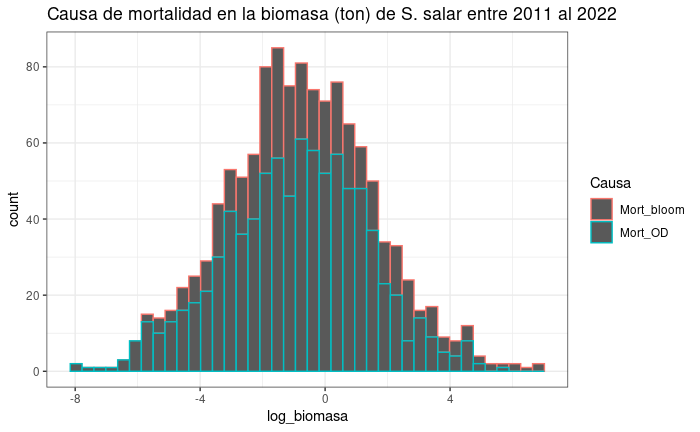
\includegraphics[width=0.9\linewidth]{Histograma_biomasa_muerta_causa} 

}

\caption{Histograma biomasa muerta (toneladas) por causa}\label{fig:unnamed-chunk-1}
\end{figure}
\end{frame}

\begin{frame}{\textbf{Datos faltantes y datos atípicos: Boxplot}}
\protect\hypertarget{datos-faltantes-y-datos-atuxedpicos-boxplot}{}
\begin{itemize}
\item
  Boxplot consideró la causa de muerte sobre la biomasa de peces entre
  el 2011 al 2022.
\item
  Datos faltantes para la causa de mortalidad por bloom entre el periodo
  2011 a 2022.
\item
  Valores atípicos presente en las dos causas de mortalidad.
\end{itemize}
\end{frame}

\begin{frame}{\textbf{BOXPLOT}}
\protect\hypertarget{boxplot}{}
\begin{figure}

{\centering \includegraphics[width=0.9\linewidth]{boxplot_biomasa_muerta_año} 

}

\caption{Boxplot biomasa muerta por año y causa}\label{fig:unnamed-chunk-2}
\end{figure}
\end{frame}

\begin{frame}{\textbf{Análisis exploratorio de los datos: Plot}}
\protect\hypertarget{anuxe1lisis-exploratorio-de-los-datos-plot}{}
\begin{itemize}
\item
  Se evidencia sobre la ocurrencia de un evento temporal puntual que
  generó una alta mortalidad en la biomasa de salmones.
\item
  Año 2021 presentó la mayor biomasa de salmones muertos siendo afectada
  por la \textbf{acción de bloom de algas}.
\item
  Año 2021 presentó la mayor mortalidad registrada históricamente en
  este barrio (log biomasa muerta \textgreater{} 5).
\end{itemize}
\end{frame}

\begin{frame}{\textbf{Relación biomasa muerta y las semanas que se
reportó mortalidad}}
\protect\hypertarget{relaciuxf3n-biomasa-muerta-y-las-semanas-que-se-reportuxf3-mortalidad}{}
\begin{figure}

{\centering 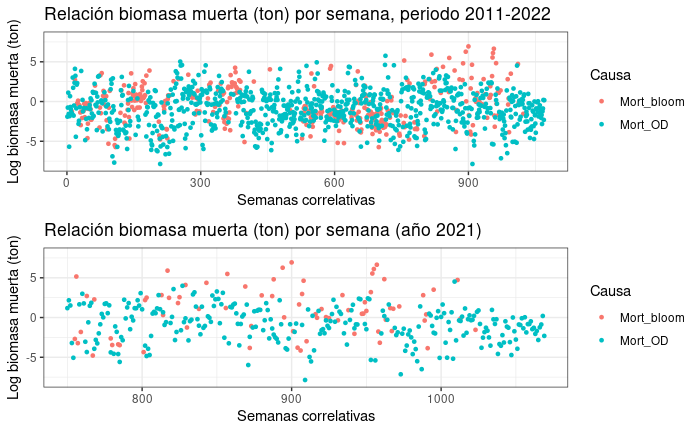
\includegraphics[width=0.9\linewidth]{Biomasa_muerta_semana_causa} 

}

\caption{Biomasa muerta por semana y causa}\label{fig:unnamed-chunk-3}
\end{figure}
\end{frame}

\begin{frame}{\textbf{Análisis exploratorio de los datos: Mortalidad
bloom vs OD}}
\protect\hypertarget{anuxe1lisis-exploratorio-de-los-datos-mortalidad-bloom-vs-od}{}
\begin{itemize}
\item
  Mayor biomasa muerta es por causa de bloom de algas, alcanzando 16
  toneledas en los ultimos 10 años.
\item
  Mortalidad por OD alcanza las 4.1 toneladas.
\item
  Peso promedio de los salmnes muertos fue de 3.1 kilogramos.
\end{itemize}
\end{frame}

\begin{frame}{\textbf{Tabla resumen de la biomasa muerta por causa}}
\protect\hypertarget{tabla-resumen-de-la-biomasa-muerta-por-causa}{}
\begin{table}

\caption{\label{tab:unnamed-chunk-4}Resumen de la biomasa muerta (toneladas) para la especie S. salar por causa entre los años 2011 al 2021}
\centering
\begin{tabular}[t]{l|r|r|r|r|r|r}
\hline
Causa & N & Promedio & DE & Mediana & Mín & Máx\\
\hline
Mort\_bloom & 360 & 16.184949 & 82.38176 & 0.4478442 & 0.0032292 & 1031.4452\\
\hline
Mort\_OD & 864 & 4.071008 & 16.81336 & 0.4349179 & 0.0003860 & 316.1441\\
\hline
\end{tabular}
\end{table}
\end{frame}

\begin{frame}{\textbf{Análisis estadísitico de los datos: Modelo lineal
simple}}
\protect\hypertarget{anuxe1lisis-estaduxedsitico-de-los-datos-modelo-lineal-simple}{}
\begin{itemize}
\item
  \textbf{Modelo de regresión lineal simple} con los factores centro,
  semanas y años.
\item
  Modelos de regresión lineal simple con los factores fueron
  estadísticamente significativos (p \textless{} 0.05), pero con un bajo
  ajuste o R\^{}2 ajustado menor al 7\%.
\end{itemize}
\end{frame}

\begin{frame}{\textbf{Hipótesis modelo lineal simple}}
\protect\hypertarget{hipuxf3tesis-modelo-lineal-simple}{}
\begin{itemize}
\tightlist
\item
  Basado en estos modelos de regresión simple se rechaza hipótesis nula
  que postulaba:
\end{itemize}

\textbf{Hipótesis nula (H0)}: Existe similitud en la biomasa muerta
entre centros/semanas/años.

\textbf{Hipótesis alternativa (H1)}: No existe similitud en la biomasa
muerta entre centros/semanas/años.
\end{frame}

\begin{frame}{\textbf{Hipótesis modelo lineal múltiple}}
\protect\hypertarget{hipuxf3tesis-modelo-lineal-muxfaltiple}{}
\begin{itemize}
\tightlist
\item
  Para el \textbf{modelo de regresión múltiple} se postularon las
  siguientes hipótesis:
\end{itemize}

\textbf{\textsubscript{H0}}: \$ \beta\_\{j\} = 0 ; j= 1,2,\ldots, k \$

\textbf{\textsubscript{H1}}: \$ \beta\_\{j\} \ne 0 ; j= 1,2,\ldots, k \$

\begin{itemize}
\tightlist
\item
  El modelo cumplió con los tres supuestos: linealidad, homogeneidad de
  varianza y normalidad.
\end{itemize}
\end{frame}

\begin{frame}{\textbf{Análisis estadísitico de los datos: Ajuste modelo
lineal múltiple}}
\protect\hypertarget{anuxe1lisis-estaduxedsitico-de-los-datos-ajuste-modelo-lineal-muxfaltiple}{}
\begin{itemize}
\item
  La modelación integró los factores causa, centro, año, mes y la
  inetracción entre causa y año.
\item
  Modelo nos estrega como resultado coeficientes distintos de cero, por
  lo tanto, se rechaza la HO (valores p menores al 5\%).
\item
  El R\^{}2 ajustado de esta modelación múltiple correspondió al 23\%.
\end{itemize}
\end{frame}

\begin{frame}{\textbf{Análisis de varianza (ANOVA)}}
\protect\hypertarget{anuxe1lisis-de-varianza-anova}{}
\begin{table}
\centering
\begin{tabular}[t]{l|r|r|r|r|r}
\hline
  & Df & Sum Sq & Mean Sq & F value & Pr(>F)\\
\hline
Causa & 1 & 63.15504 & 63.155039 & 14.624314 & 0.0001381\\
\hline
año & 11 & 248.97448 & 22.634044 & 5.241187 & 0.0000000\\
\hline
centro\_id & 22 & 615.45852 & 27.975387 & 6.478040 & 0.0000000\\
\hline
mes & 11 & 665.02969 & 60.457244 & 13.999607 & 0.0000000\\
\hline
Causa:año & 7 & 175.41762 & 25.059660 & 5.802868 & 0.0000012\\
\hline
Residuals & 1171 & 5056.95851 & 4.318496 & NA & NA\\
\hline
\end{tabular}
\end{table}
\end{frame}

\begin{frame}{\textbf{Comparación de modelos por RSS y AIC}}
\protect\hypertarget{comparaciuxf3n-de-modelos-por-rss-y-aic}{}
\begin{itemize}
\item
  Crietrios de anova de residuales (RSS) y Akaike Information Criterion
  (AIC)
\item
  Ambos criterios sugieren al modelo lineal múltiple con la mejor
  predicción y ajuste (23\%).
\end{itemize}

Quitting from lines 201-202 (Presentacion\_Felipe\_Tucca.Rmd) Error in
anova(modelo1\_anova1\_centro, modelo2\_anova2\_mes,
modelo3\_anova3\_año, : object `modelo1\_anova1\_centro' not found
Calls: \ldots{} eval\_with\_user\_handlers -\textgreater{} eval
-\textgreater{} eval -\textgreater{} \%\textgreater\% -\textgreater{}
pander -\textgreater{} anova

Quitting from lines 205-207 (Presentacion\_Felipe\_Tucca.Rmd) Error in
AIC(modelo1\_anova1\_centro, modelo2\_anova2\_mes, modelo3\_anova3\_año,
: object `modelo1\_anova1\_centro' not found Calls: \ldots{}
eval\_with\_user\_handlers -\textgreater{} eval -\textgreater{} eval
-\textgreater{} \%\textgreater\% -\textgreater{} pander -\textgreater{}
AIC
\end{frame}

\begin{frame}{\textbf{Interpretación y y conclusiones del trabajo}}
\protect\hypertarget{interpretaciuxf3n-y-y-conclusiones-del-trabajo}{}
\begin{itemize}
\item
  Análisis exploratorio muestra mayor mortalidad de la biomasa de peces
  en el barrio por bloom.
\item
  Mortalidad por baja de OD presenta mayor frecuencia.
\item
  Se realizó ANOVA con un vía de criterio de clasificación para los
  factores centro de cultivo, semanas y años con ajustes menores al 7\%.
\item
  Modelo lineal múltiple agrupó todas los factores mostrando un
  significancia menor al 5\%.
\item
  El ajuste de la predicción de la variable biomasa muerta fue de un
  23\% (modelo regresión múltiple)
\item
  Análisis comparativo por RSS y AIC entre modelos determinó que la
  \textbf{regresión lineal múltiple representa una mejor predicción}
\end{itemize}
\end{frame}

\end{document}
